Intro text.
\section{Computational Details}
Text.
\section{$G_{1g}$ Spectrum}
The isotriplet strange $G_{1g}$ symmetry channel is parity-positive and consists of spins $\frac{1}{2}$, $\frac{7}{2}$, $\frac{9}{2}$, and beyond. In this channel, we expect to see the physical $\Sigma$, the $\Sigma(1660)$, and the $\Sigma(2030)$, which have spins $\frac{1}{2}$, $\frac{1}{2}$, and $\frac{7}{2}$, respectively. In addition to these single-hadron states, we expect to see many multi-hadron states. Reliably extracting finite-volume single-hadron states that correspond to resonances in infinite-volume requires the use of multi-hadron operators, since we expect a resonance to have some overlap onto its decay products. While it would be ideal to compute many-hadron correlators, computing correlators for states with greater than two hadrons is prohibitively expensive, so we limit ourselves to using operators which are designed to create at most two hadrons.

In general, we start with a large basis of operators, and \emph{prune} out those which are either too noisy or not sufficiently linearly independent. For the single-hadron operators, we started with a large basis 16 operators, and pruned our set down to just 7. For the two-hadron operators, we started with a basis of 35 operators, and pruned our set down to just 21. The final basis of single- and two-hadron operators used to extract the spectrum in this channel are given in Table~\ref{table:g1g_ops}. Just as in Sec.~\ref{sec:a0}, we make use of variationally improved single-hadron operators. That is, first diagonalize in the subspace of single-hadron operators to form linear combinations which overlap more independently onto the single-hadron states of interest, in order to aid in level identification.

\begin{table}
    \centering
    \begin{tabular}{l|l}
        \textbf{Single-Hadron Operators} & \textbf{Two-Hadron Operators} \\
        \hline
        $\Sigma_{G_{1g}}^{DDI0}$ & $\pi(0)_{A_{1u}^-}^{SS0}\Lambda(0)_{G_{1u}}^{SS2}$\\
        $\Sigma_{G_{1g}}^{DDI22}$ & $\pi(0)_{A_{1u}^-}^{SS0}\Lambda(0)_{G_{1u}}^{SS3}$\\
        $\Sigma_{G_{1g}}^{DDL55}$ & $\pi(1)_{A_2^-}^{SS1}\Lambda(1)_{G_1}^{SS1}$\\
        $\Sigma_{G_{1g}}^{SS2}$ & $\pi(2)_{A_2^-}^{SS0}\Lambda(2)_{G}^{SS0}$\\
        $\Sigma_{G_{1g}}^{SS3}$ & $\pi(3)_{A_2^-}^{SS0}\Lambda(3)_{G}^{SS0}$\\
        $\Sigma_{G_{1g}}^{TDT65}$ & $\pi(1)_{A_2^-}^{SS0}\Sigma(1)_{G_1}^{SS0}$\\
        $\Sigma_{G_{1g}}^{TDT72}$ & $\pi(1)_{A_2^-}^{SS1}\Sigma(1)_{G_1}^{SS0}$\\
        & $\pi(1)_{A_2^-}^{SS1}\Sigma(1)_{G_1}^{SS2}$\\
        & $\pi(2)_{A_2^-}^{SS0}\Sigma(2)_{G}^{SS1}$\\
        & $\pi(3)_{A_2^-}^{SS0}\Sigma(3)_{G}^{SS4}$\\
        & $\overline K(1)_{A_1}^{SS2}N(1)_{G_1}^{SS0}$\\
        & $\overline K(1)_{A_2}^{SS0}N(1)_{G_1}^{SS0}$\\
        & $\overline K(1)_{A_2}^{SS1}N(1)_{G_1}^{SS0}$\\
        & $\overline K(1)_{E}^{SS2}N(1)_{G_1}^{SS0}$\\
        & $\overline K(4)_{A_2}^{SS1}N(4)_{G_1}^{SS0}$\\
        & $\overline K(2)_{A_2}^{SS0}N(2)_{G}^{SS0}$\\
        & $\overline K(2)_{A_2}^{SS1}N(2)_{G}^{SS0}$\\
        & $\overline K(3)_{A_2}^{SS0}N(3)_{G}^{SS0}$\\
        & $\overline K(1)_{A_2}^{SS1}\Delta(1)_{G_1}^{SS0}$\\
        & $K(1)_{A_2}^{SS1}\Xi(1)_{G_1}^{SS0}$\\
        & $\eta(1)_{A_2^+}^{SS1}\Sigma(1)_{G_1}^{SS0}$
    \end{tabular}
    \caption{Operators used in the isotriplet strange $G_{1g}$ symmetry sector.}\label{table:g1g_ops}
\end{table}

The spectrum obtained in terms of the kaon mass (obtained from the fit given in Ch.~\ref{ch:tetraquarks}) is shown in Fig.~\ref{fig:g1g_spectrum}. Correlator fits are shown in Fig.~\ref{fig:g1g_fits}.

\begin{figure}
    \centering
    \hspace*{-0.5in}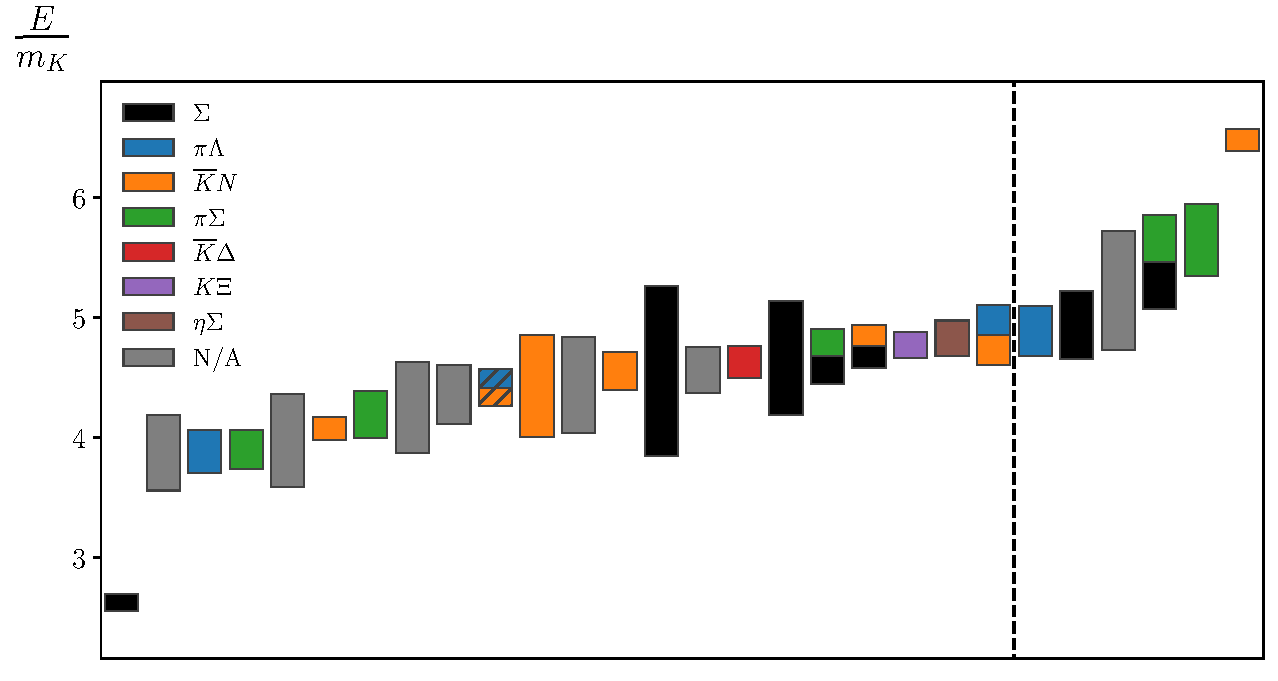
\includegraphics[width=\textwidth]{figures/sigmas/g1g/staircase_mk.pdf}
    \caption{The full spectrum for the isosinglet strange $G_{1g}$ channel, obtained by fitting the energies and overlap factors of the diagonalized correlator matrix. A qualitative attempt at level identification is made by determining, for each operator, which level overlaps maximally with the state created by that operator. If a level does not overlap maximally with the any operator's state, we denote its flavor content as ``N/A''. Because we expect a single-hadron resonance to have significant overlap with potential decay products, we also use hatching to denote any level which has an overlap of $\geq 70\%$ of the maximum overlap with a single-hadron operator.}\label{fig:g1g_spectrum}
\end{figure}

\begin{figure}
    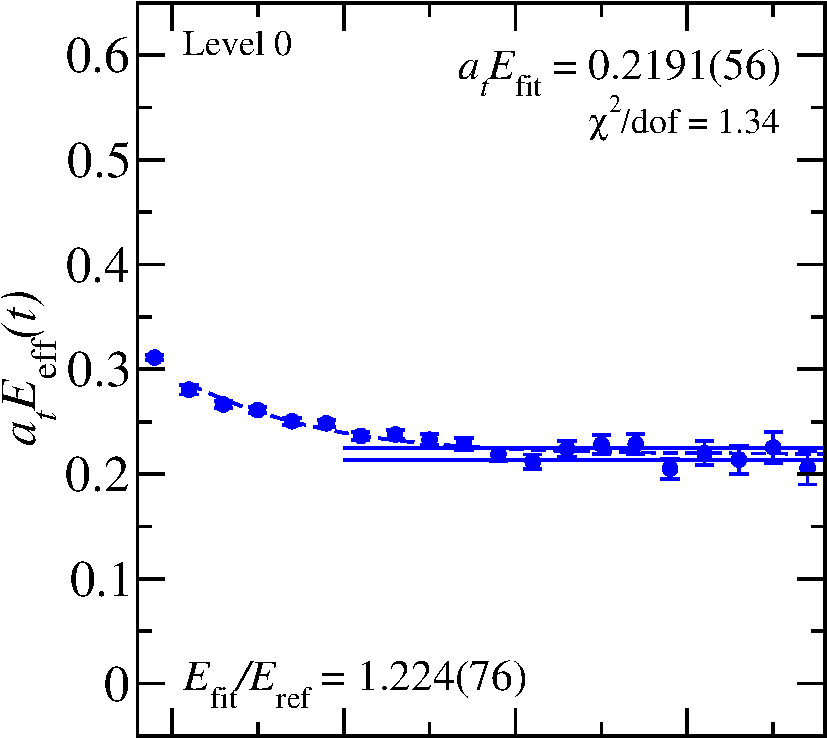
\includegraphics[width=0.215\textwidth]{figures/sigmas/g1g/fits/fit_0.pdf}
    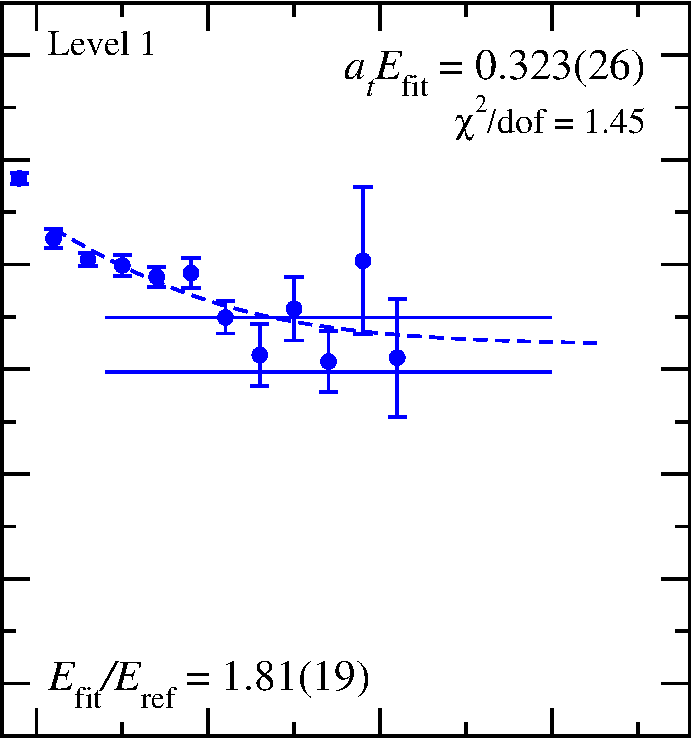
\includegraphics[width=0.18\textwidth]{figures/sigmas/g1g/fits/fit_7.pdf}
    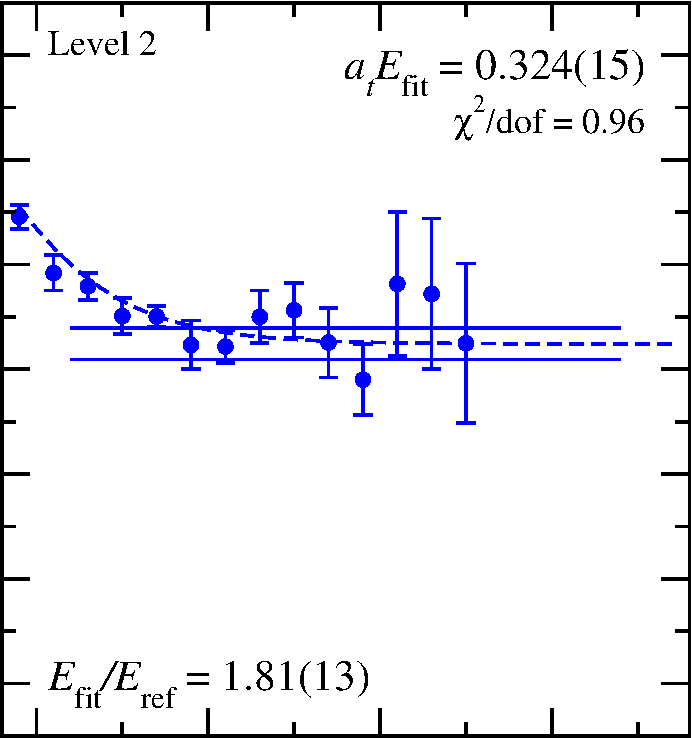
\includegraphics[width=0.18\textwidth]{figures/sigmas/g1g/fits/fit_3.pdf}
    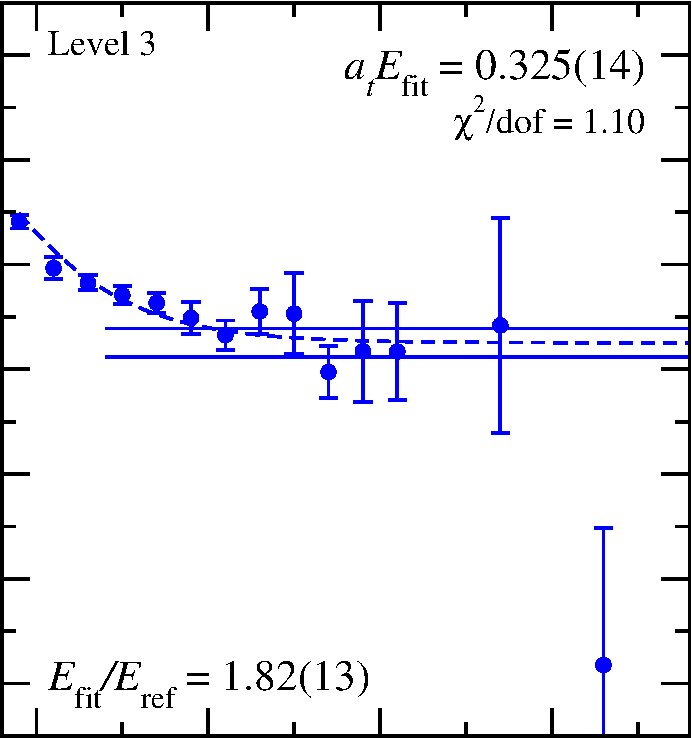
\includegraphics[width=0.18\textwidth]{figures/sigmas/g1g/fits/fit_4.pdf}
    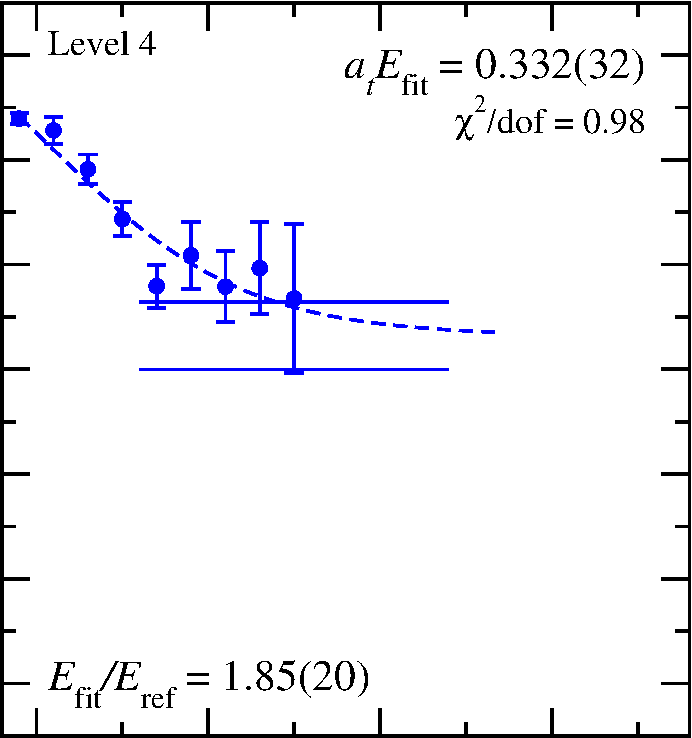
\includegraphics[width=0.18\textwidth]{figures/sigmas/g1g/fits/fit_21.pdf}\\
    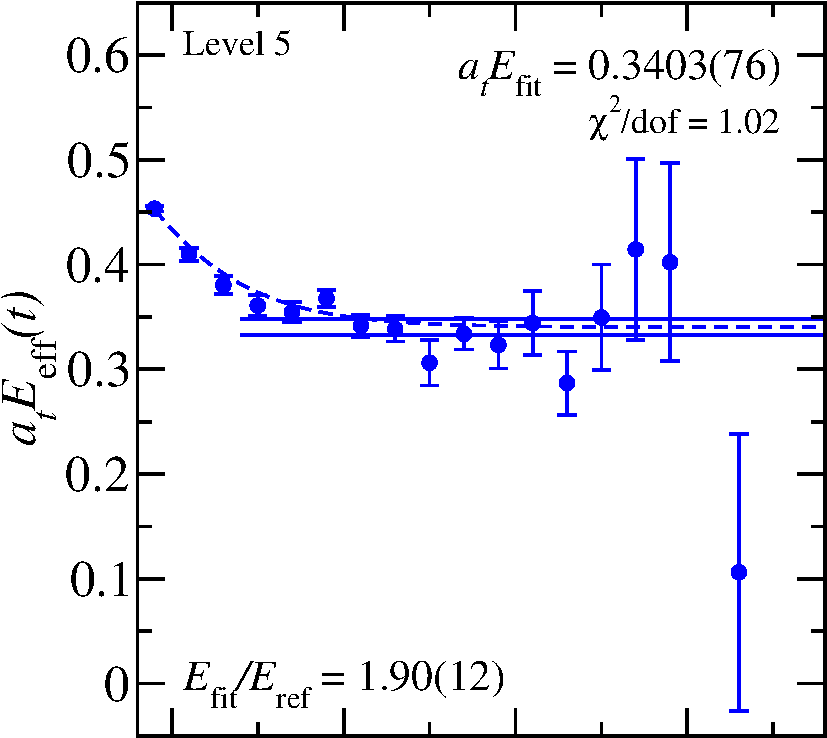
\includegraphics[width=0.215\textwidth]{figures/sigmas/g1g/fits/fit_5.pdf}
    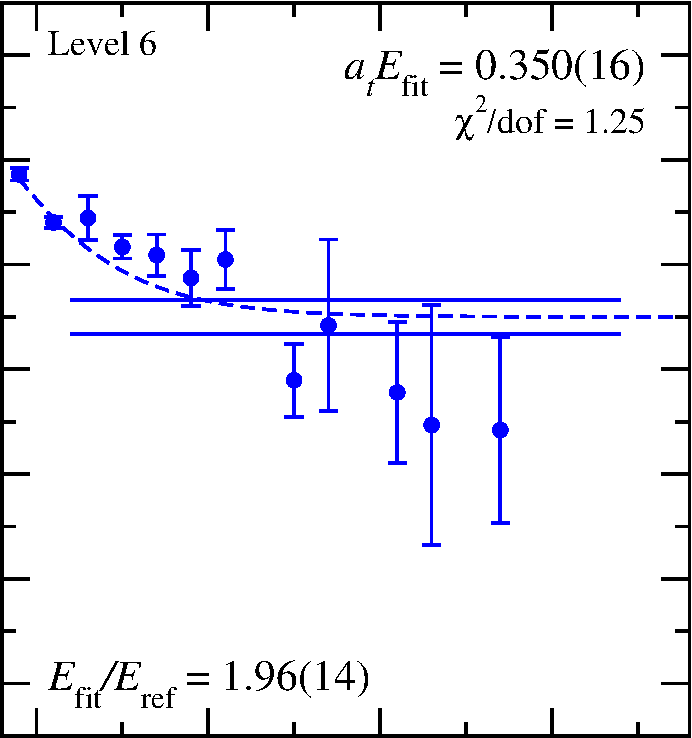
\includegraphics[width=0.18\textwidth]{figures/sigmas/g1g/fits/fit_9.pdf}
    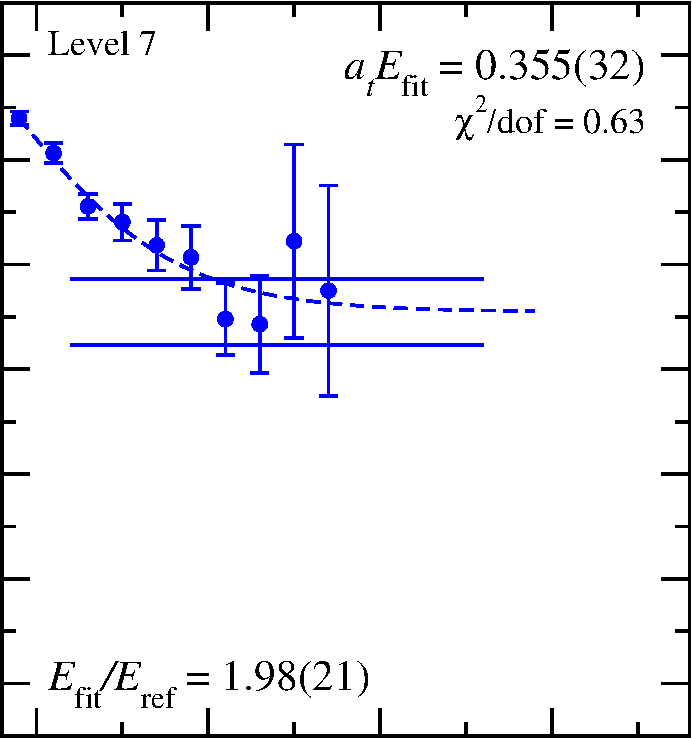
\includegraphics[width=0.18\textwidth]{figures/sigmas/g1g/fits/fit_19.pdf}
    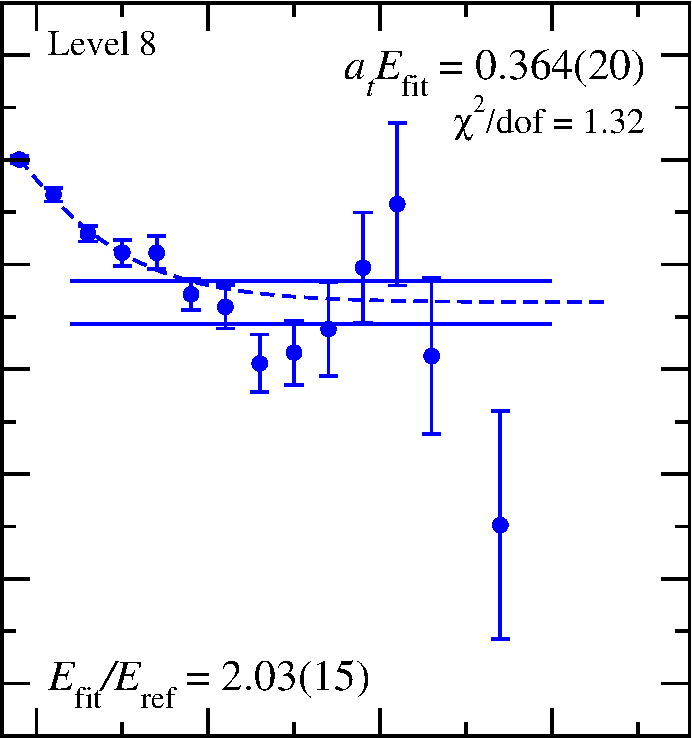
\includegraphics[width=0.18\textwidth]{figures/sigmas/g1g/fits/fit_14.pdf}
    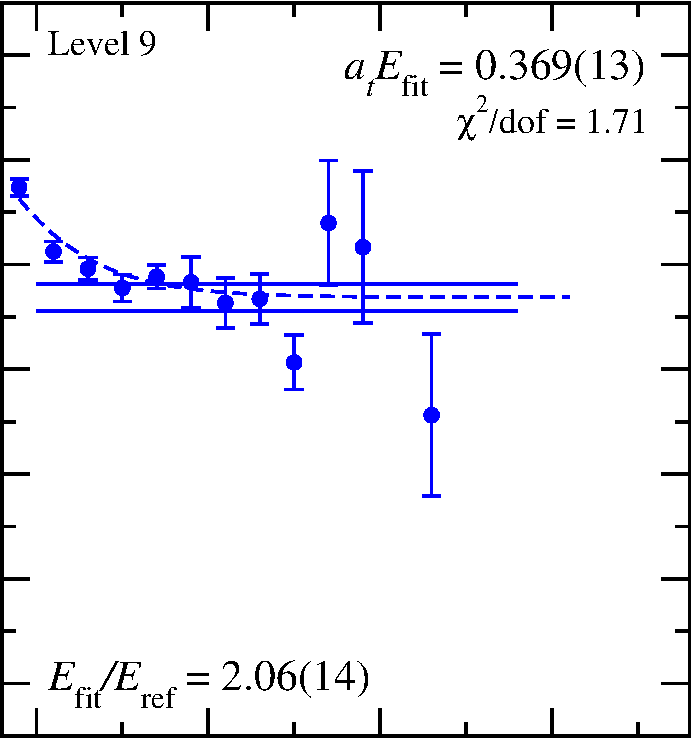
\includegraphics[width=0.18\textwidth]{figures/sigmas/g1g/fits/fit_6.pdf}\\
    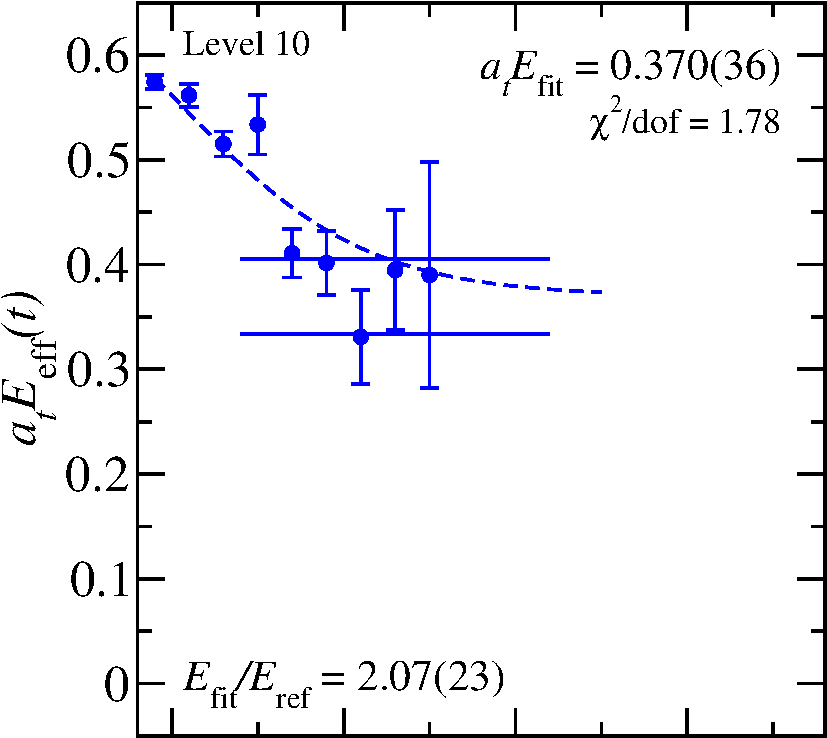
\includegraphics[width=0.215\textwidth]{figures/sigmas/g1g/fits/fit_23.pdf}
    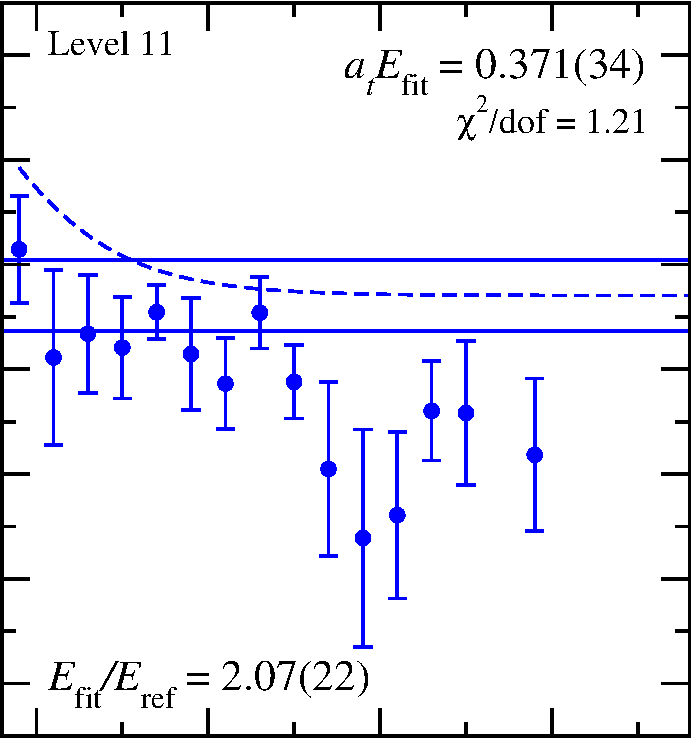
\includegraphics[width=0.18\textwidth]{figures/sigmas/g1g/fits/fit_1.pdf}
    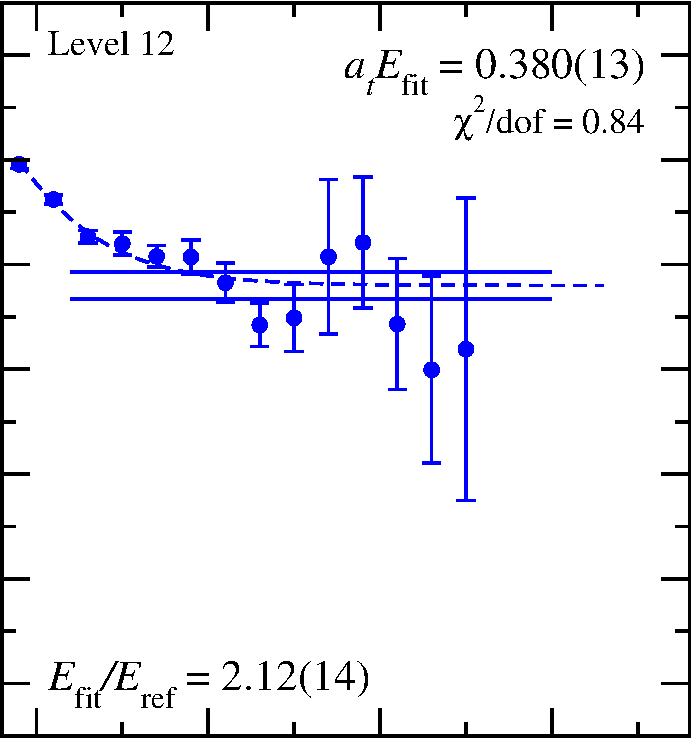
\includegraphics[width=0.18\textwidth]{figures/sigmas/g1g/fits/fit_13.pdf}
    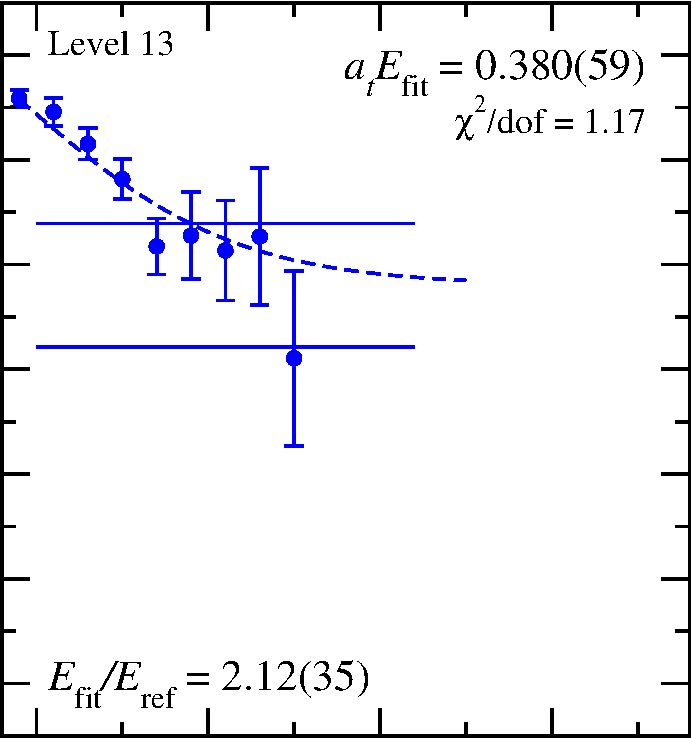
\includegraphics[width=0.18\textwidth]{figures/sigmas/g1g/fits/fit_22.pdf}
    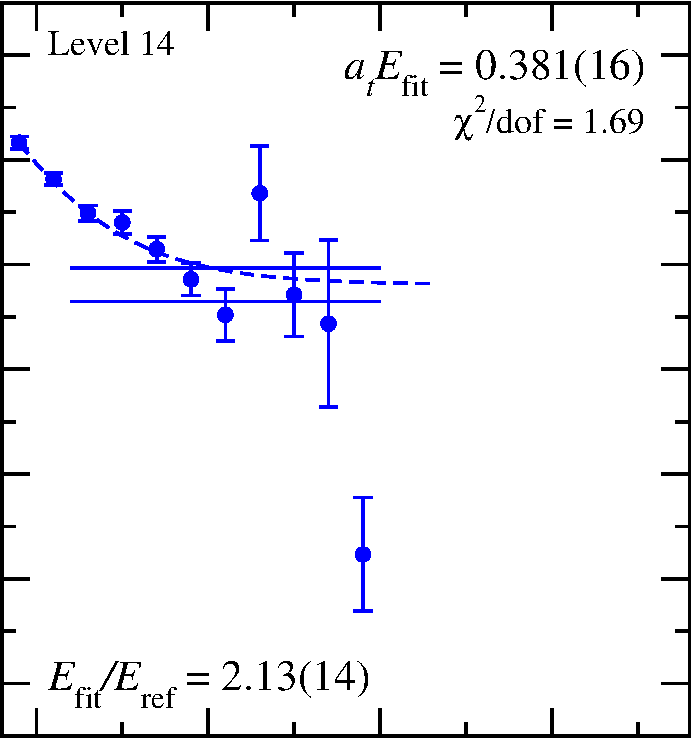
\includegraphics[width=0.18\textwidth]{figures/sigmas/g1g/fits/fit_16.pdf}\\
    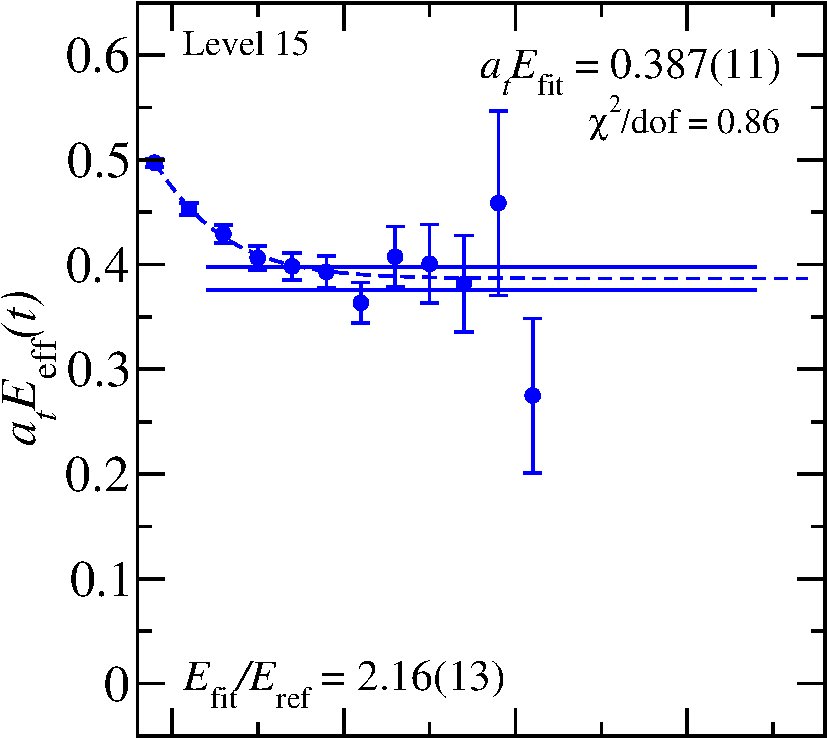
\includegraphics[width=0.215\textwidth]{figures/sigmas/g1g/fits/fit_11.pdf}
    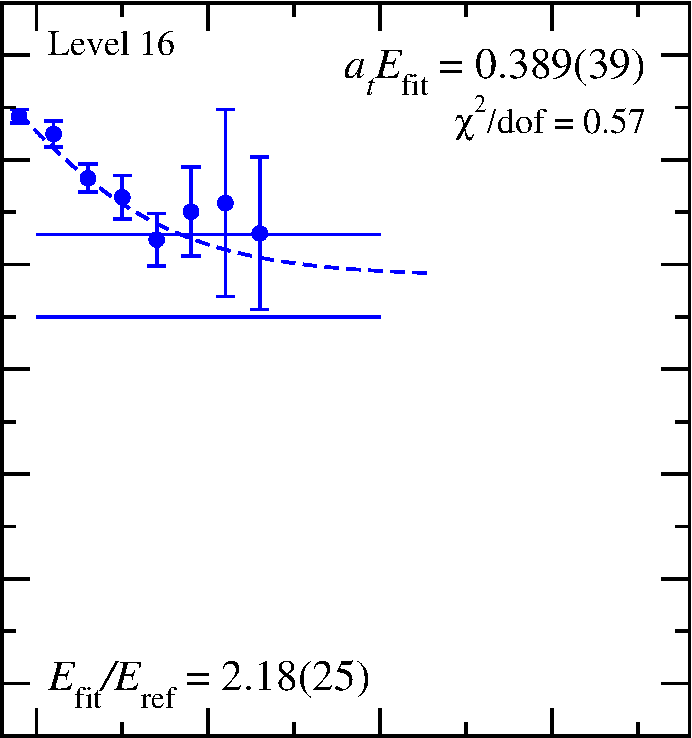
\includegraphics[width=0.18\textwidth]{figures/sigmas/g1g/fits/fit_20.pdf}
    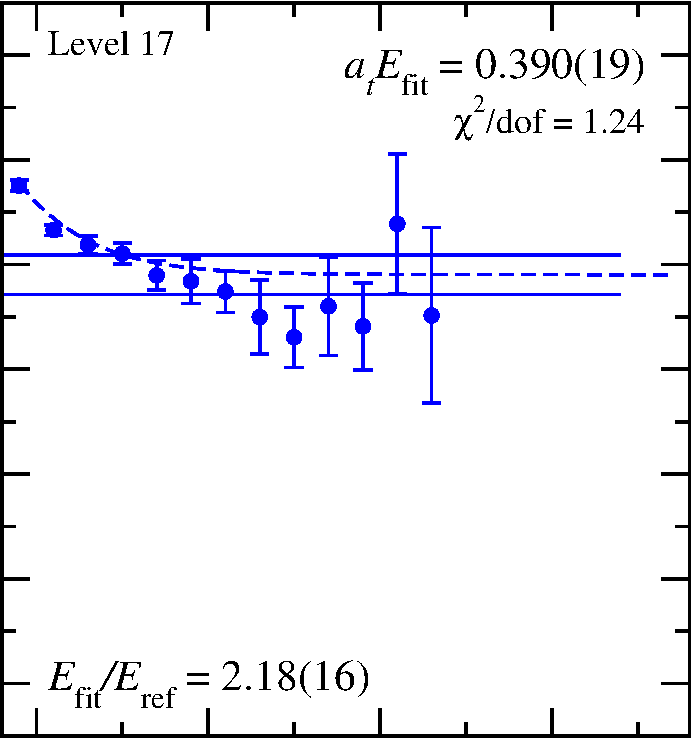
\includegraphics[width=0.18\textwidth]{figures/sigmas/g1g/fits/fit_8.pdf}
    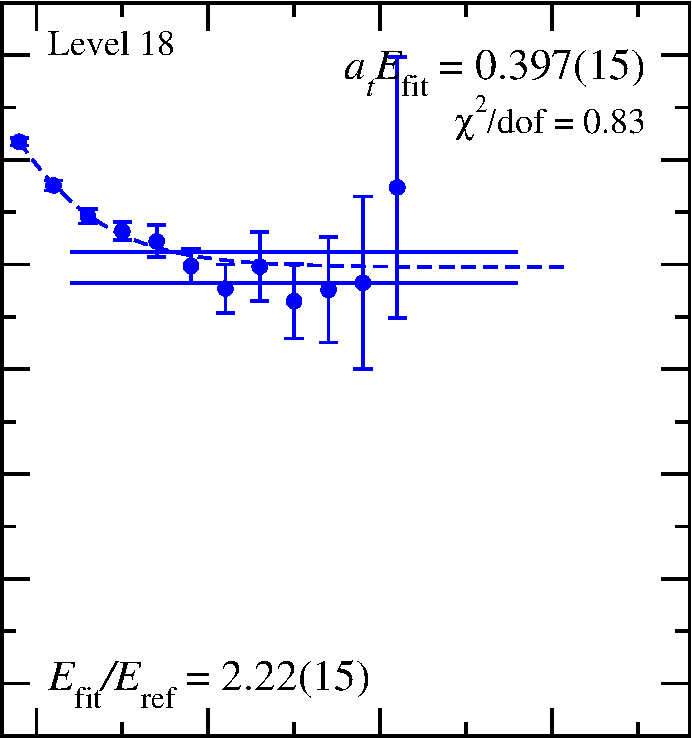
\includegraphics[width=0.18\textwidth]{figures/sigmas/g1g/fits/fit_15.pdf}
    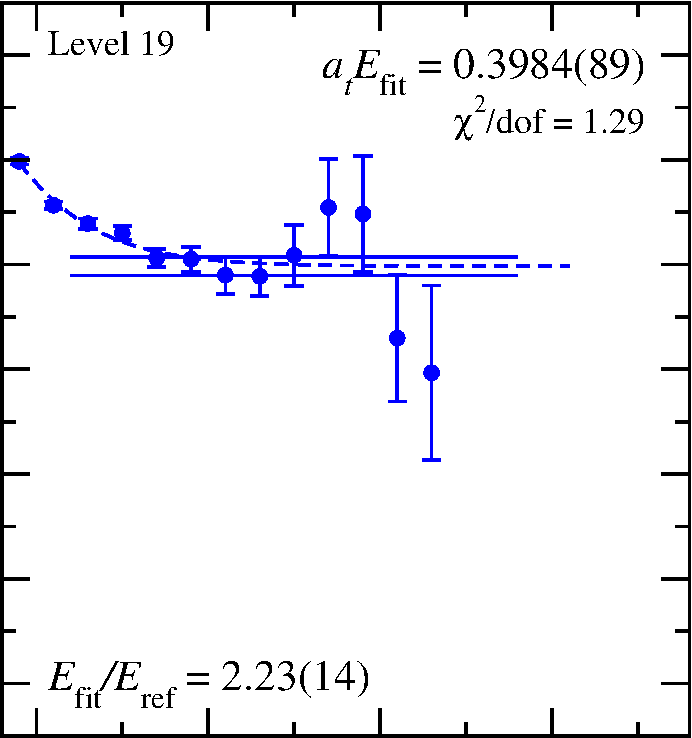
\includegraphics[width=0.18\textwidth]{figures/sigmas/g1g/fits/fit_12.pdf}\\
    \raisebox{0.35cm}{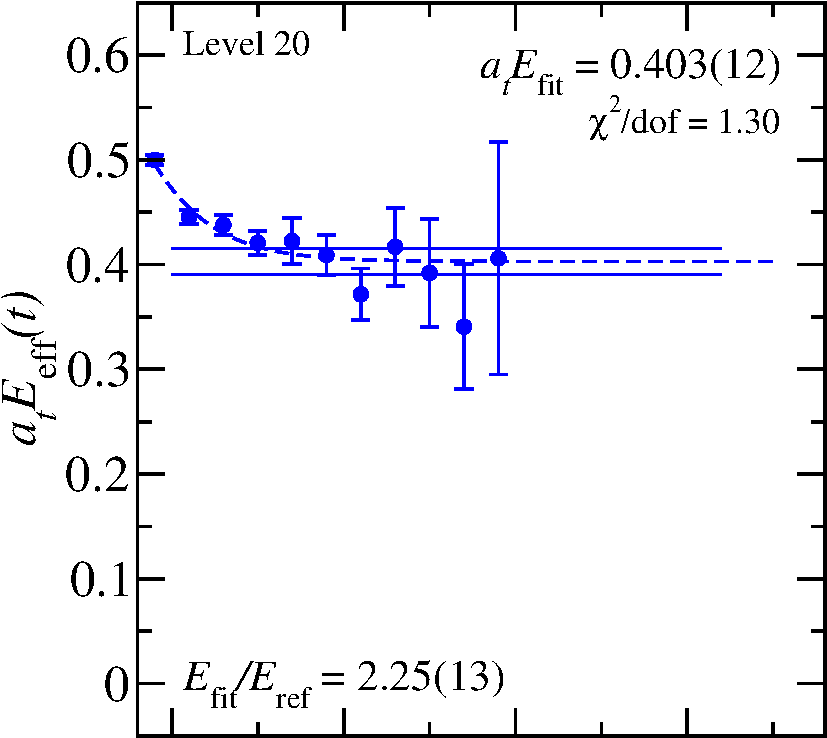
\includegraphics[width=0.215\textwidth]{figures/sigmas/g1g/fits/fit_10.pdf}}
    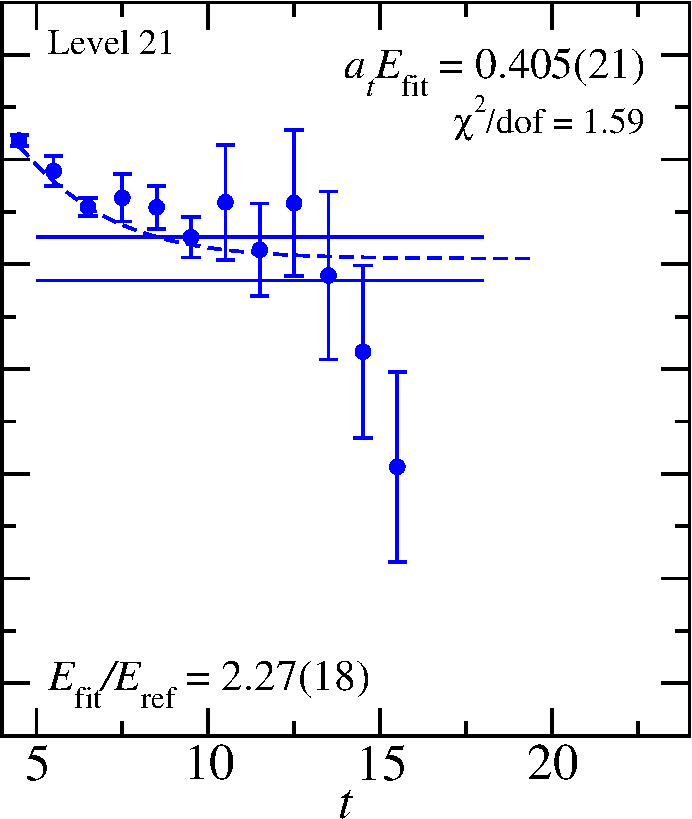
\includegraphics[width=0.18\textwidth]{figures/sigmas/g1g/fits/fit_17.pdf}
    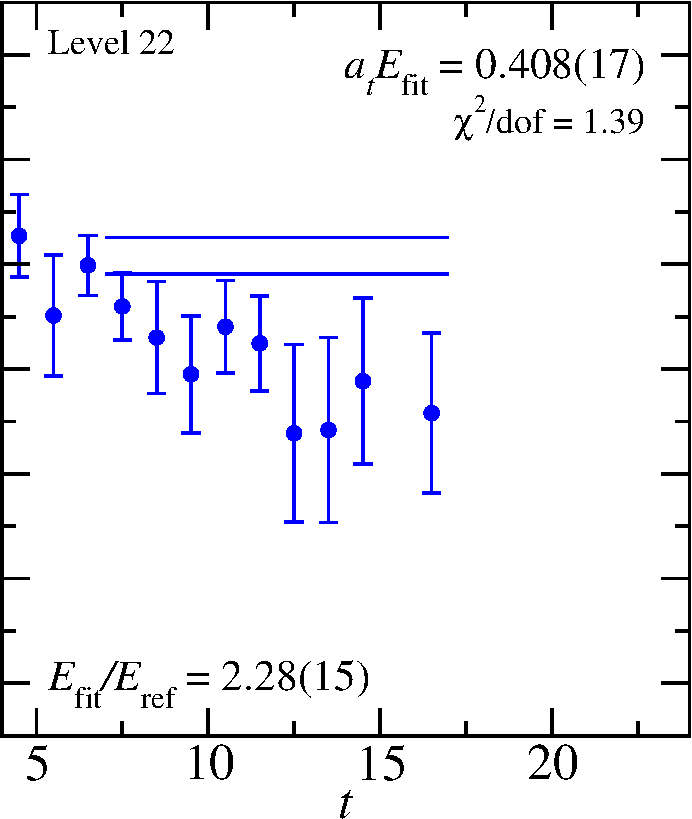
\includegraphics[width=0.18\textwidth]{figures/sigmas/g1g/fits/fit_2.pdf}
    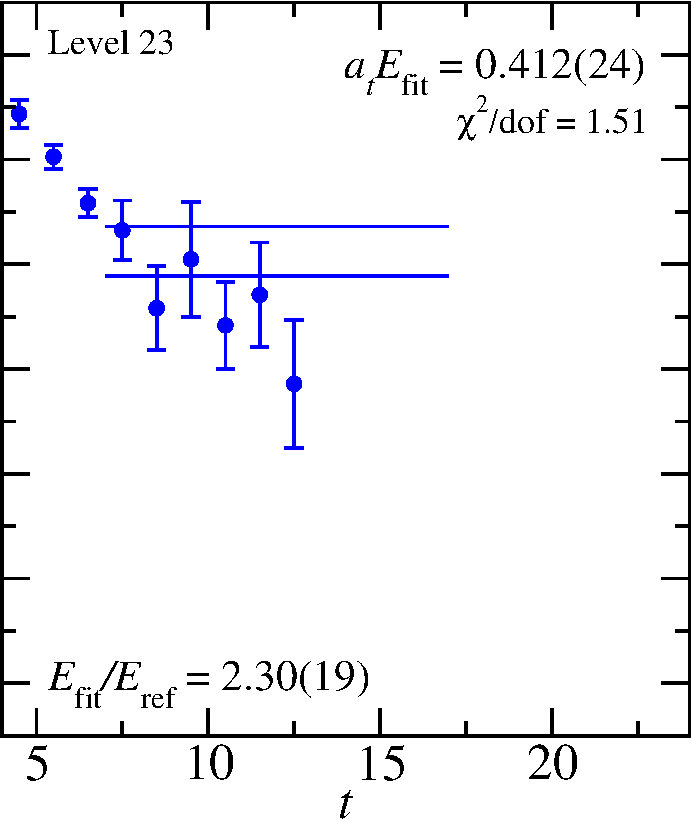
\includegraphics[width=0.18\textwidth]{figures/sigmas/g1g/fits/fit_18.pdf}
    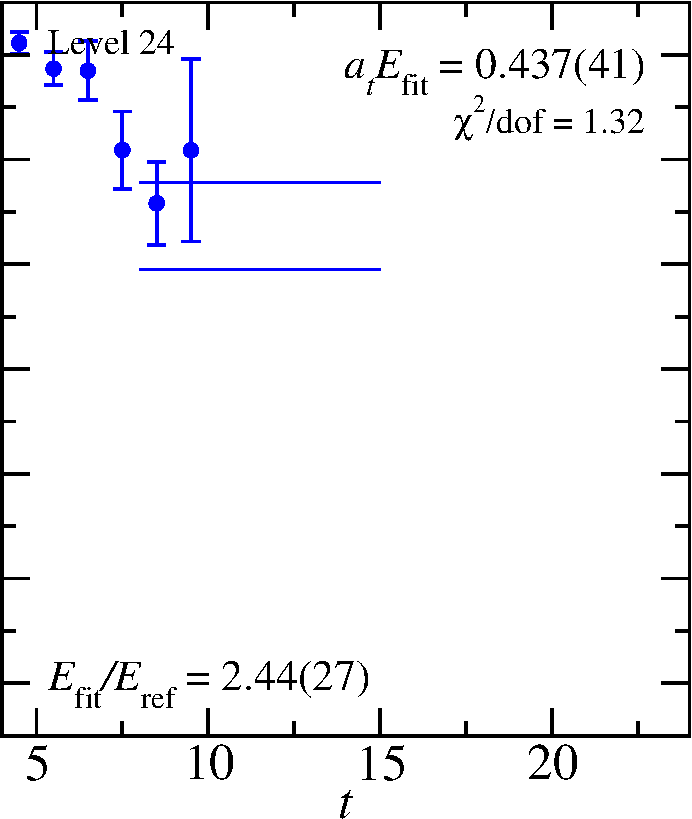
\includegraphics[width=0.18\textwidth]{figures/sigmas/g1g/fits/fit_25.pdf}\\[-0.35cm]
    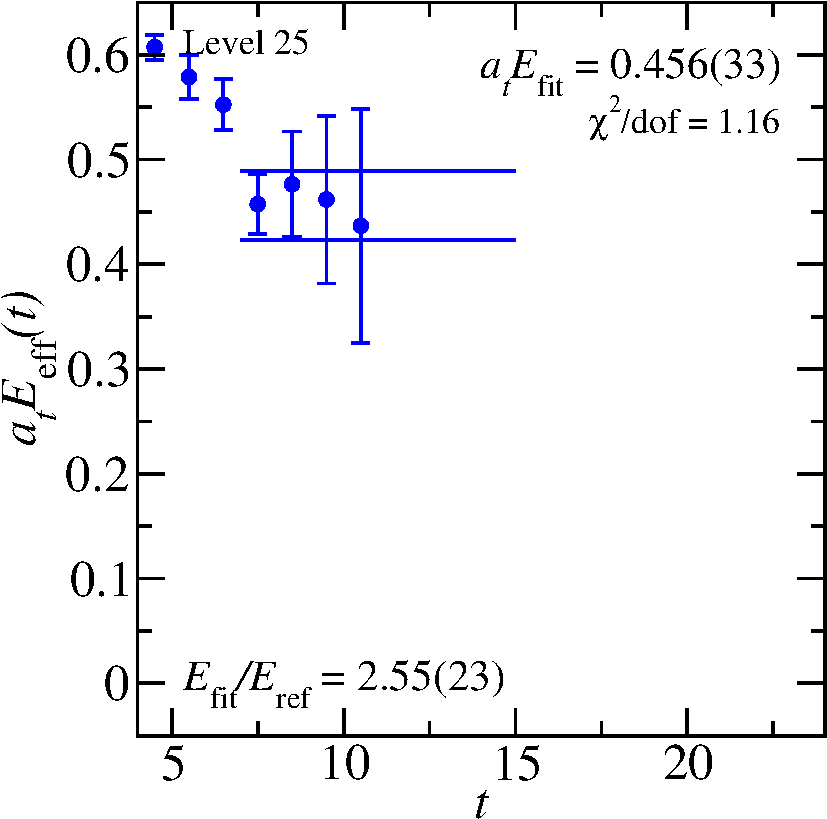
\includegraphics[width=0.215\textwidth]{figures/sigmas/g1g/fits/fit_24.pdf}
    \caption{}\label{fig:g1g_fits}
\end{figure}

\begin{figure}
    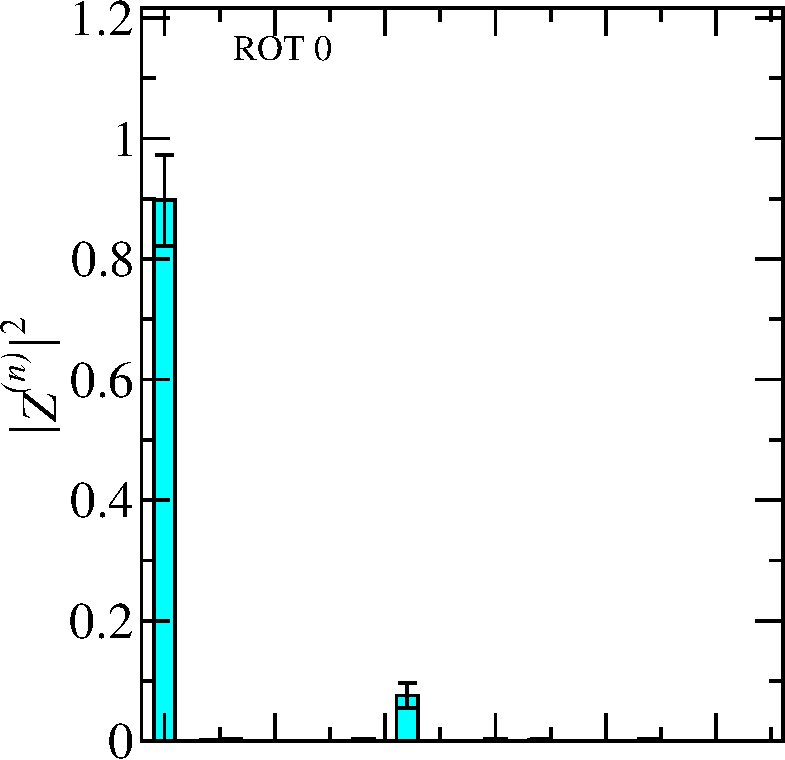
\includegraphics[width=.1975\textwidth]{figures/sigmas/g1g/zfactors/zfactor_isotriplet-S-1-P000-G1g_1-ROT-0.pdf}
    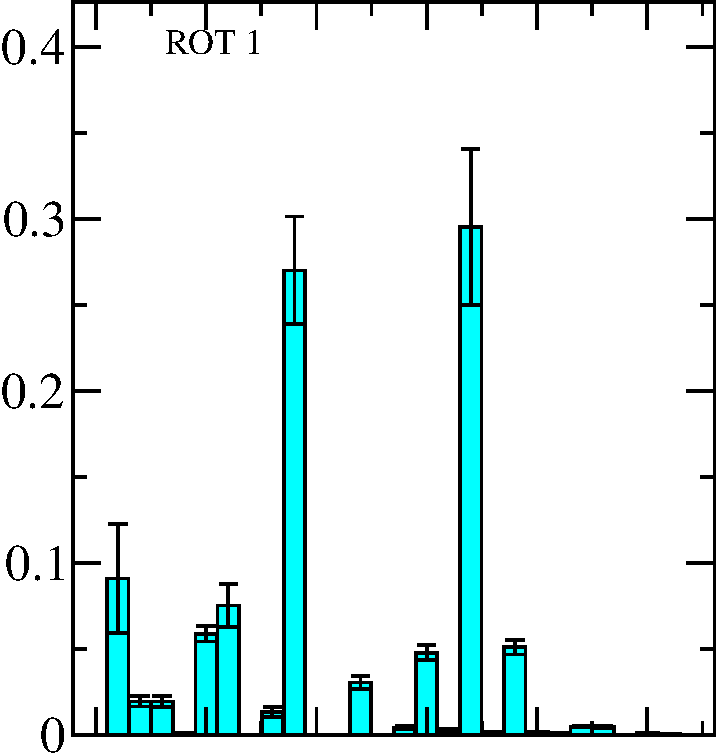
\includegraphics[width=.18\textwidth]{figures/sigmas/g1g/zfactors/zfactor_isotriplet-S-1-P000-G1g_1-ROT-1.pdf}
    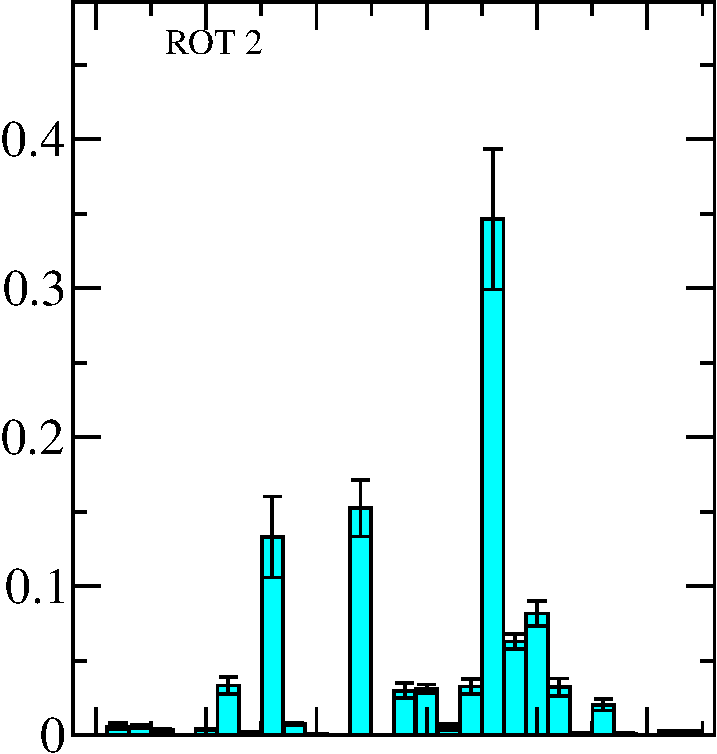
\includegraphics[width=.18\textwidth]{figures/sigmas/g1g/zfactors/zfactor_isotriplet-S-1-P000-G1g_1-ROT-2.pdf}
    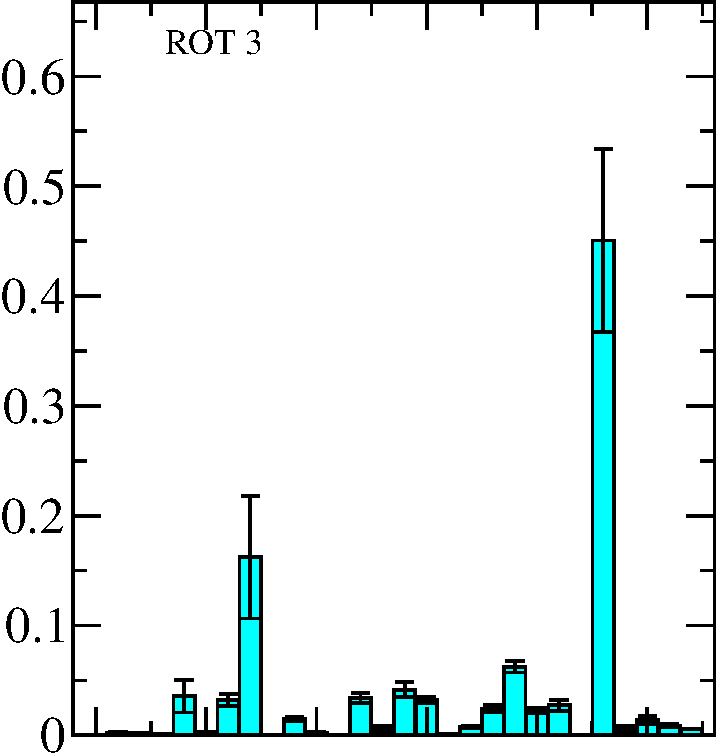
\includegraphics[width=.18\textwidth]{figures/sigmas/g1g/zfactors/zfactor_isotriplet-S-1-P000-G1g_1-ROT-3.pdf}
    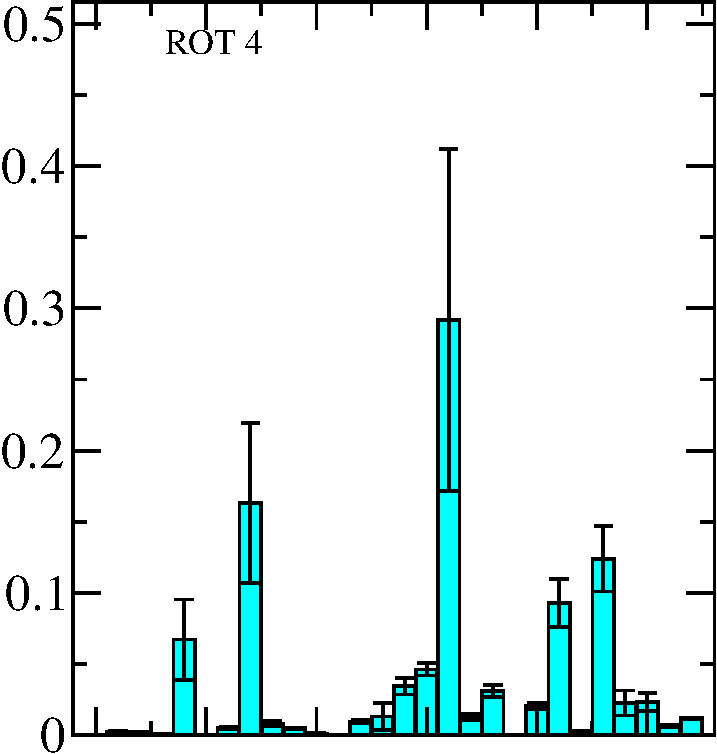
\includegraphics[width=.18\textwidth]{figures/sigmas/g1g/zfactors/zfactor_isotriplet-S-1-P000-G1g_1-ROT-4.pdf}\\
    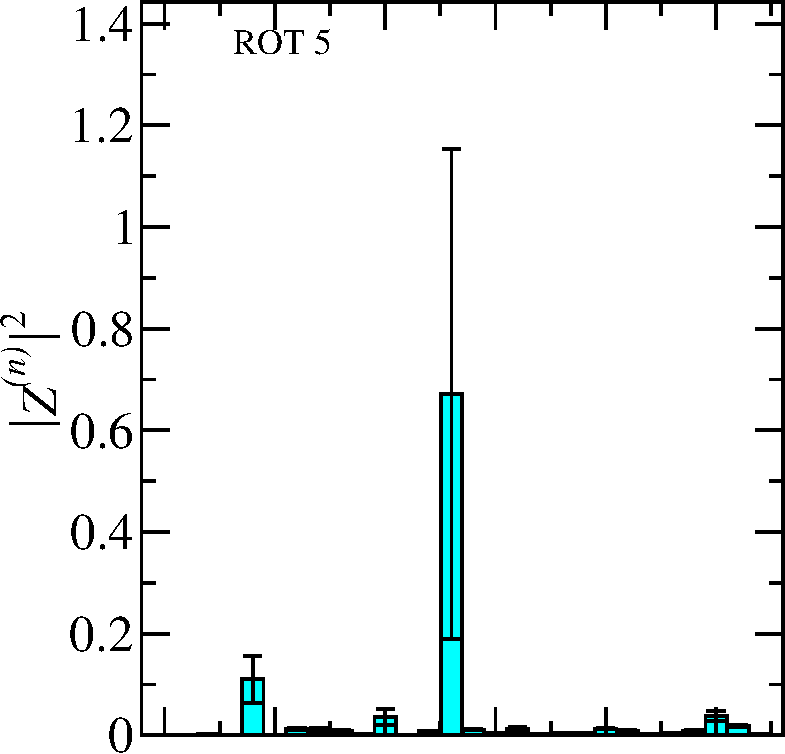
\includegraphics[width=.1975\textwidth]{figures/sigmas/g1g/zfactors/zfactor_isotriplet-S-1-P000-G1g_1-ROT-5.pdf}
    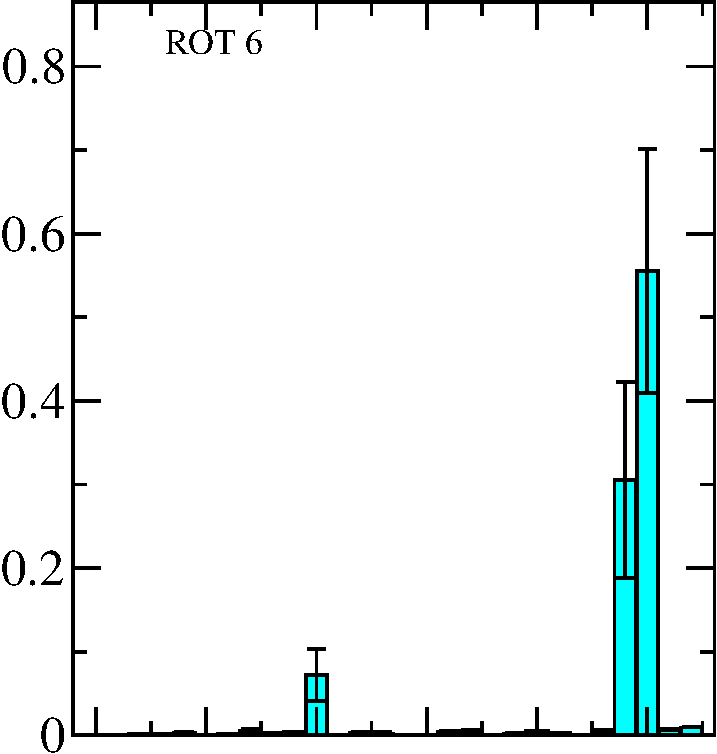
\includegraphics[width=.18\textwidth]{figures/sigmas/g1g/zfactors/zfactor_isotriplet-S-1-P000-G1g_1-ROT-6.pdf}
    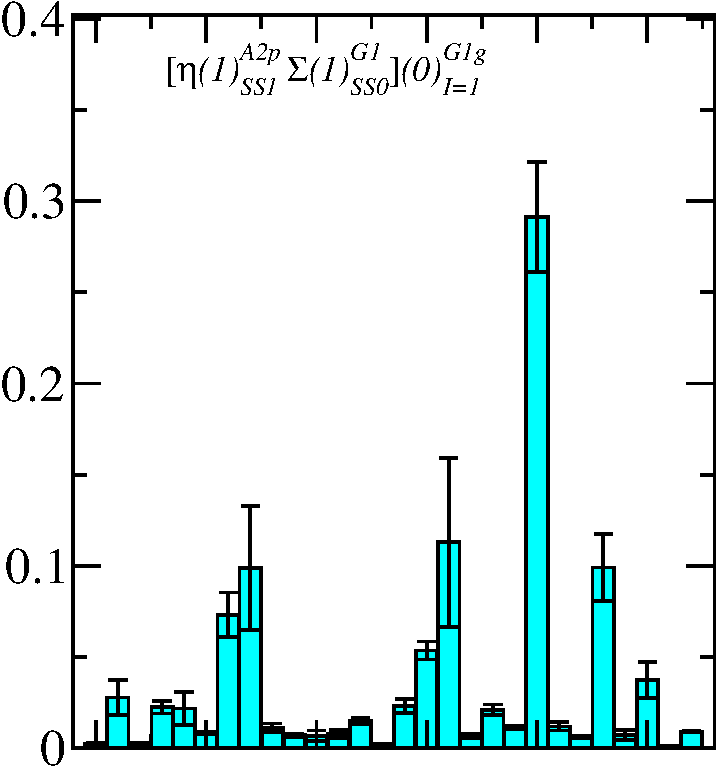
\includegraphics[width=.18\textwidth]{figures/sigmas/g1g/zfactors/zfactor_isotriplet_eta_sigma-G1g_1-P001-A2p-SS_1-P00-1-G1-SS_0.pdf}
    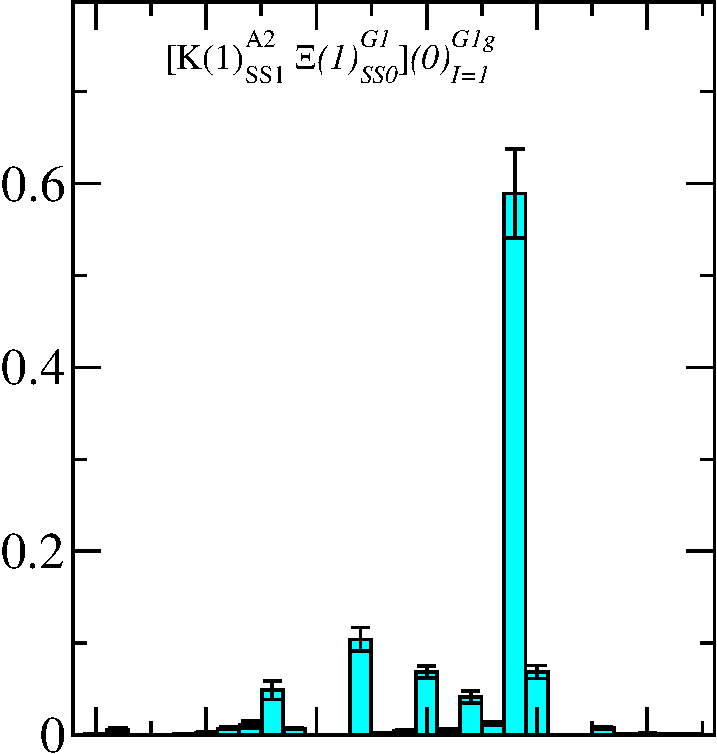
\includegraphics[width=.18\textwidth]{figures/sigmas/g1g/zfactors/zfactor_isotriplet_kaon_xi-G1g_1-P001-A2-SS_1-P00-1-G1-SS_0.pdf}
    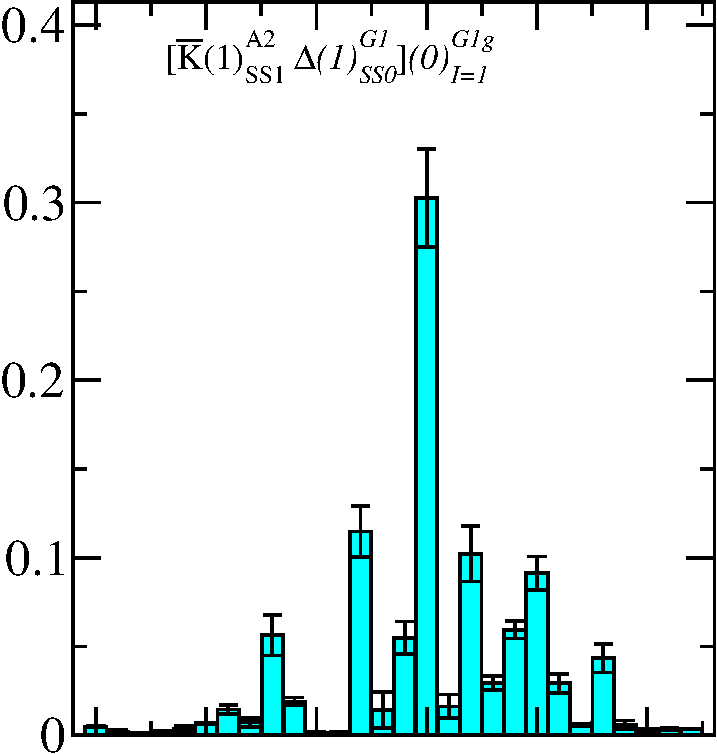
\includegraphics[width=.18\textwidth]{figures/sigmas/g1g/zfactors/zfactor_isotriplet_kbar_delta-G1g_1-P001-A2-SS_1-P00-1-G1-SS_0.pdf}\\
    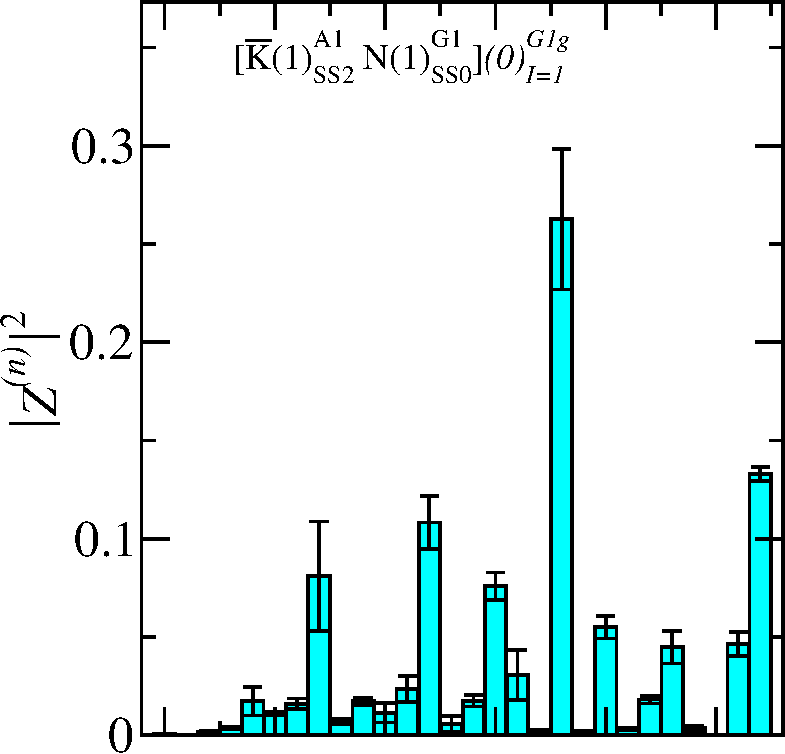
\includegraphics[width=.1975\textwidth]{figures/sigmas/g1g/zfactors/zfactor_isotriplet_kbar_nucleon-G1g_1-P001-A1-SS_2-P00-1-G1-SS_0.pdf}
    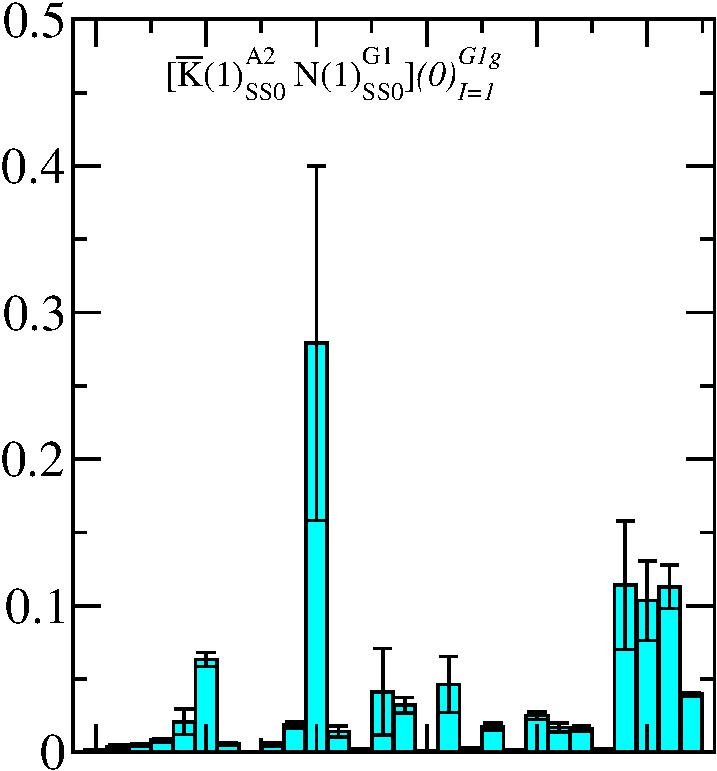
\includegraphics[width=.18\textwidth]{figures/sigmas/g1g/zfactors/zfactor_isotriplet_kbar_nucleon-G1g_1-P001-A2-SS_0-P00-1-G1-SS_0.pdf}
    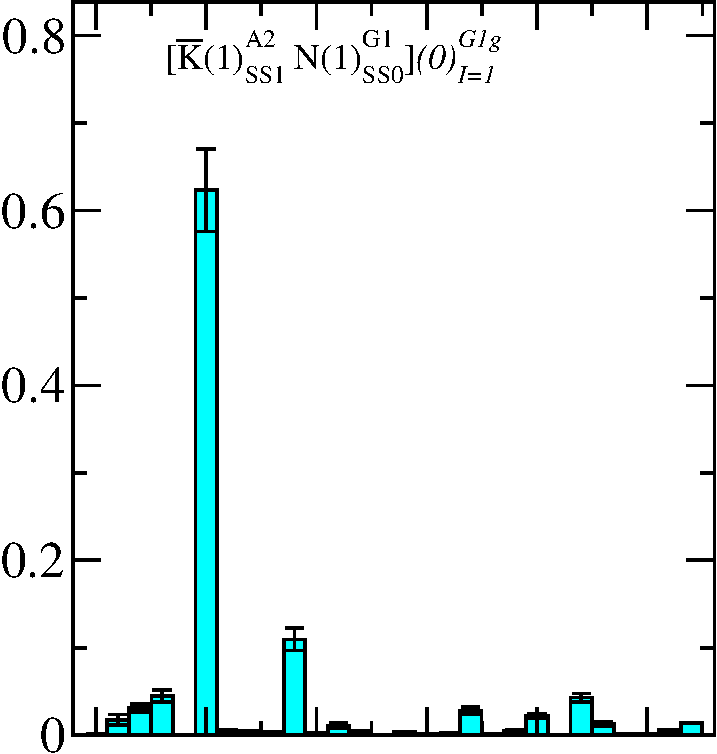
\includegraphics[width=.18\textwidth]{figures/sigmas/g1g/zfactors/zfactor_isotriplet_kbar_nucleon-G1g_1-P001-A2-SS_1-P00-1-G1-SS_0.pdf}
    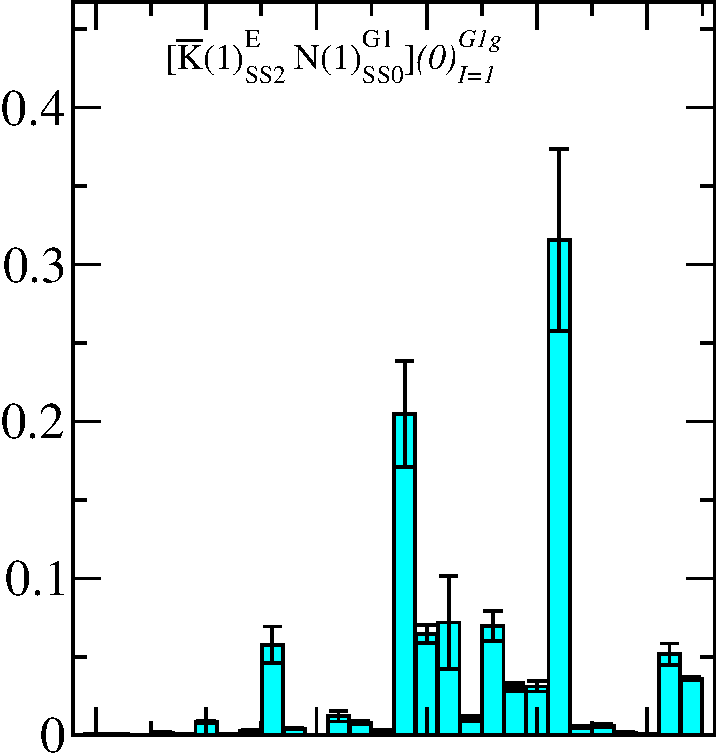
\includegraphics[width=.18\textwidth]{figures/sigmas/g1g/zfactors/zfactor_isotriplet_kbar_nucleon-G1g_1-P001-E-SS_2-P00-1-G1-SS_0.pdf}
    \hspace*{-0.1cm}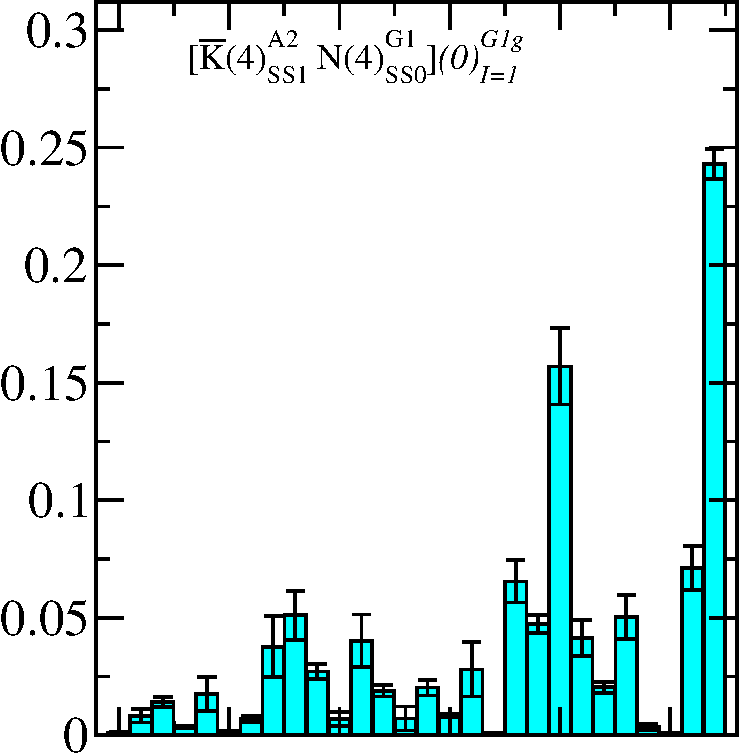
\includegraphics[width=.185\textwidth]{figures/sigmas/g1g/zfactors/zfactor_isotriplet_kbar_nucleon-G1g_1-P002-A2-SS_1-P00-2-G1-SS_0.pdf}\\
    \hspace*{-0.1cm}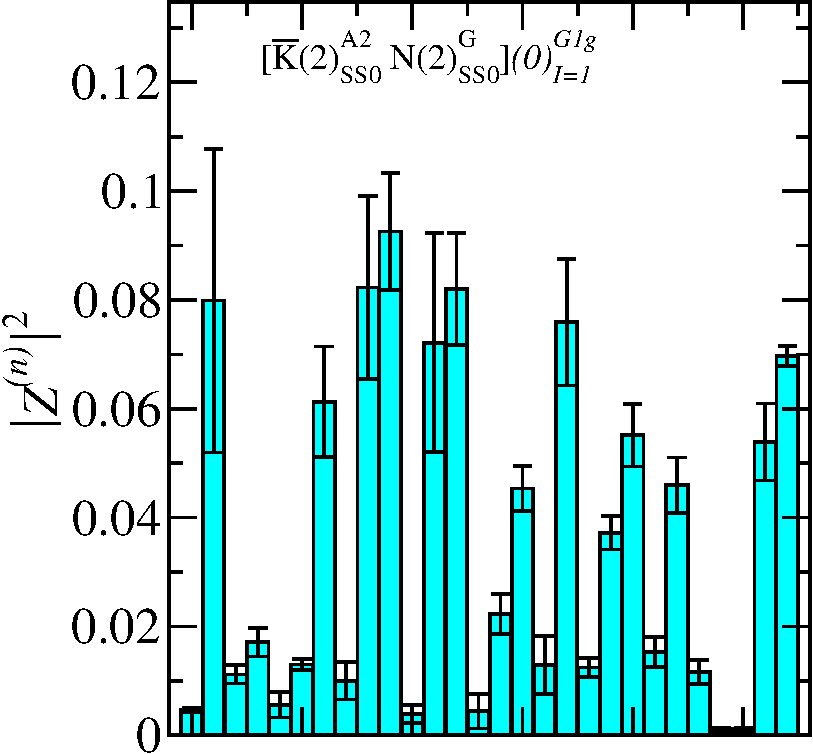
\includegraphics[width=.205\textwidth]{figures/sigmas/g1g/zfactors/zfactor_isotriplet_kbar_nucleon-G1g_1-P011-A2-SS_0-P0-1-1-G-SS_0.pdf}
    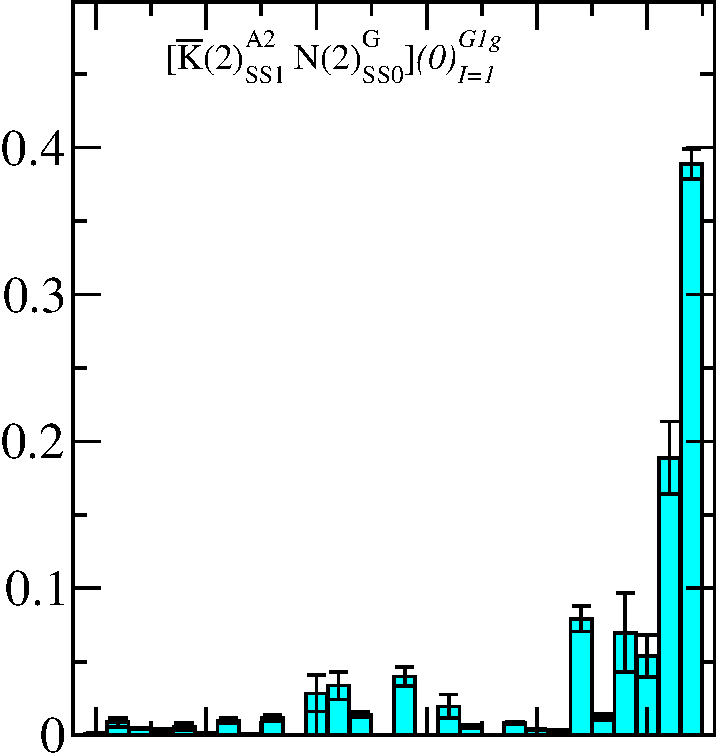
\includegraphics[width=.18\textwidth]{figures/sigmas/g1g/zfactors/zfactor_isotriplet_kbar_nucleon-G1g_1-P011-A2-SS_1-P0-1-1-G-SS_0.pdf}
    \hspace*{-0.1cm}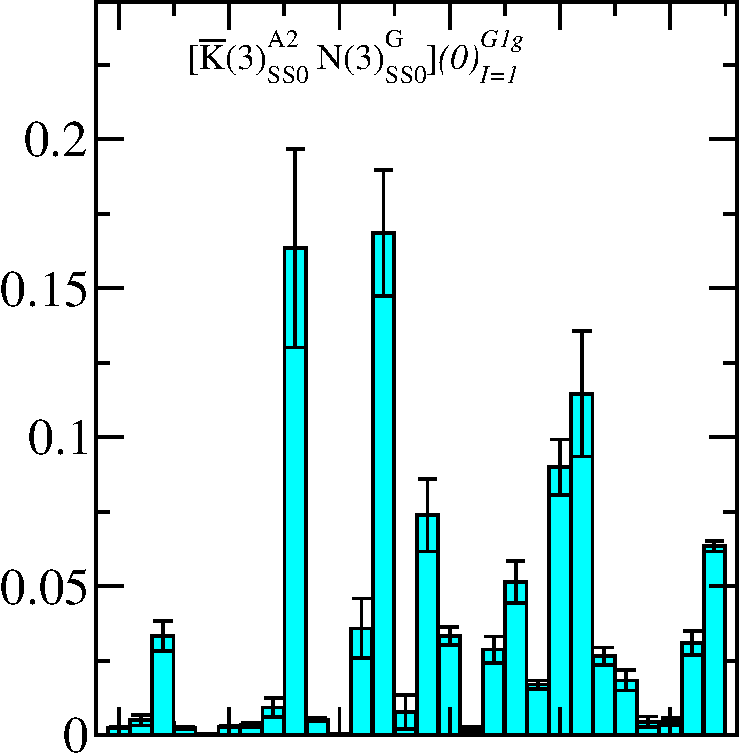
\includegraphics[width=.185\textwidth]{figures/sigmas/g1g/zfactors/zfactor_isotriplet_kbar_nucleon-G1g_1-P111-A2-SS_0-P-1-1-1-G-SS_0.pdf}
    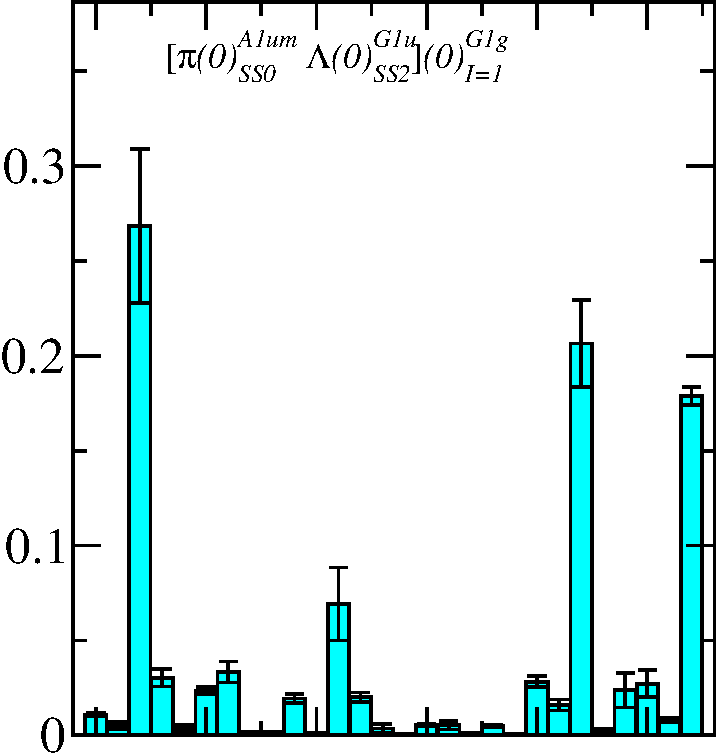
\includegraphics[width=.18\textwidth]{figures/sigmas/g1g/zfactors/zfactor_isotriplet_pion_lambda-G1g_1-P000-A1um-SS_0-P000-G1u-SS_2.pdf}
    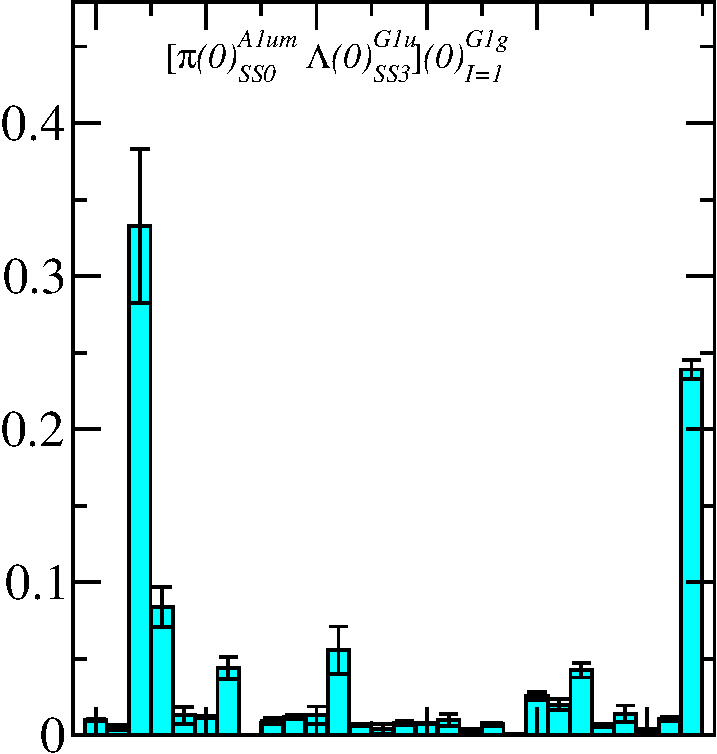
\includegraphics[width=.18\textwidth]{figures/sigmas/g1g/zfactors/zfactor_isotriplet_pion_lambda-G1g_1-P000-A1um-SS_0-P000-G1u-SS_3.pdf}\\
    \raisebox{0.5cm}{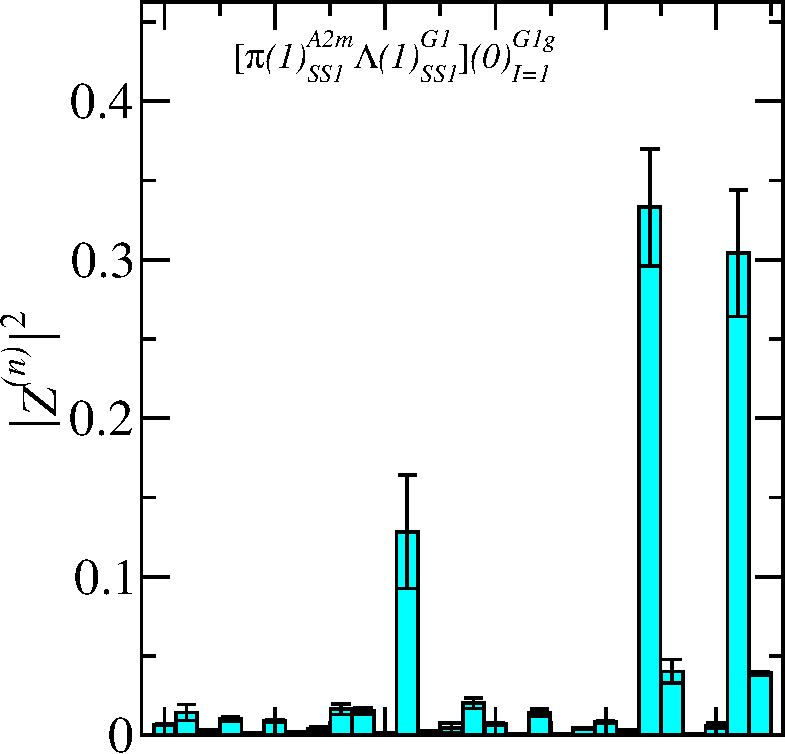
\includegraphics[width=.1975\textwidth]{figures/sigmas/g1g/zfactors/zfactor_isotriplet_pion_lambda-G1g_1-P001-A2m-SS_1-P00-1-G1-SS_1.pdf}}
    \raisebox{0.5cm}{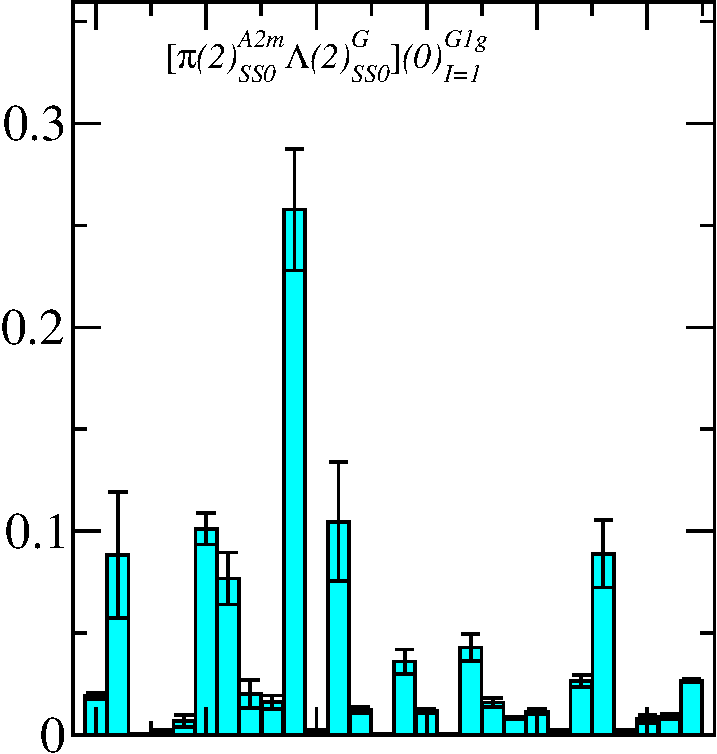
\includegraphics[width=.18\textwidth]{figures/sigmas/g1g/zfactors/zfactor_isotriplet_pion_lambda-G1g_1-P011-A2m-SS_0-P0-1-1-G-SS_0.pdf}}
    \hspace*{-0.05cm}\raisebox{0.5cm}{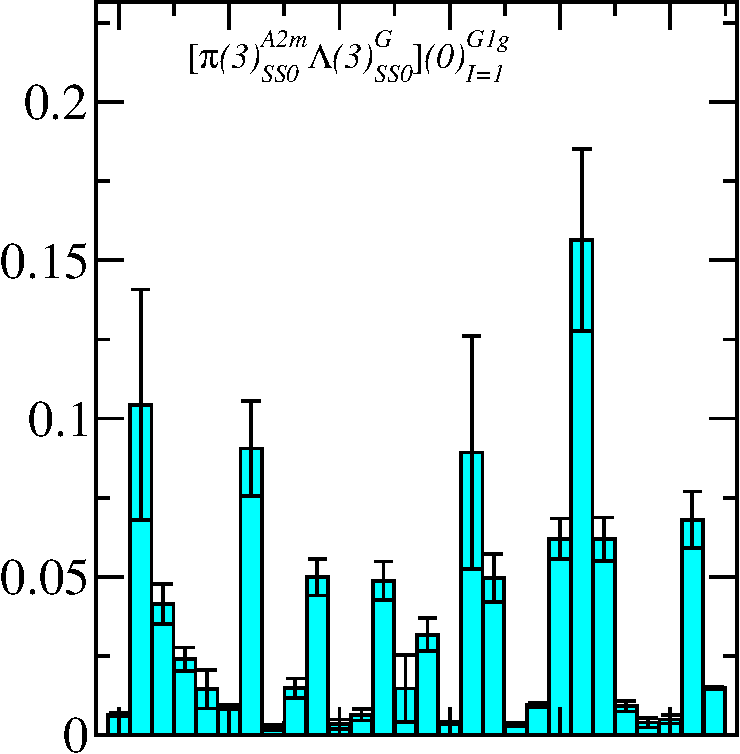
\includegraphics[width=.185\textwidth]{figures/sigmas/g1g/zfactors/zfactor_isotriplet_pion_lambda-G1g_1-P111-A2m-SS_0-P-1-1-1-G-SS_0.pdf}}
    \raisebox{0.2cm}{\includegraphics[width=.18\textwidth]{figures/sigmas/g1g/zfactors/zfactor_isotriplet_pion_sigma-G1g_1-P001-A2m-SS_0-P00-1-G1-SS_0.pdf}}
    \raisebox{0.2cm}{\includegraphics[width=.18\textwidth]{figures/sigmas/g1g/zfactors/zfactor_isotriplet_pion_sigma-G1g_1-P001-A2m-SS_1-P00-1-G1-SS_0.pdf}}\\[-0.5cm]
    \includegraphics[width=.1975\textwidth]{figures/sigmas/g1g/zfactors/zfactor_isotriplet_pion_sigma-G1g_1-P001-A2m-SS_1-P00-1-G1-SS_2.pdf}
    \hspace*{-0.06cm}\includegraphics[width=.185\textwidth]{figures/sigmas/g1g/zfactors/zfactor_isotriplet_pion_sigma-G1g_1-P011-A2m-SS_0-P0-1-1-G-SS_1.pdf}
    \hspace*{-0.06cm}\includegraphics[width=.185\textwidth]{figures/sigmas/g1g/zfactors/zfactor_isotriplet_pion_sigma-G1g_1-P111-A2m-SS_0-P-1-1-1-G-SS_4.pdf}
    \caption{}\label{fig:g1g_zfactors}
\end{figure}

\section{$G_{1u}$ Spectrum}
\section{$H_g$ Spectrum}
\section{$H_u$ Spectrum}
\section{$G_{2g}$ Spectrum}
\section{$G_{2u}$ Spectrum}